\section{Modelo en VDM++}
\label{sec:modelo}

El componente crítico del sistema, el algoritmo de búsqueda de rutas, se
especificó como una clase VDM++ denominada \texttt{Sistema}. El modelo se
organiza en tipos, una variable de instancia, funciones auxiliares y
operaciones con pre y postcondiciones. La Figura~\ref{fig:modelo} muestra
el modelo completo cargado en la VDM++ Toolbox.

\begin{figure*}[!t]
\centering
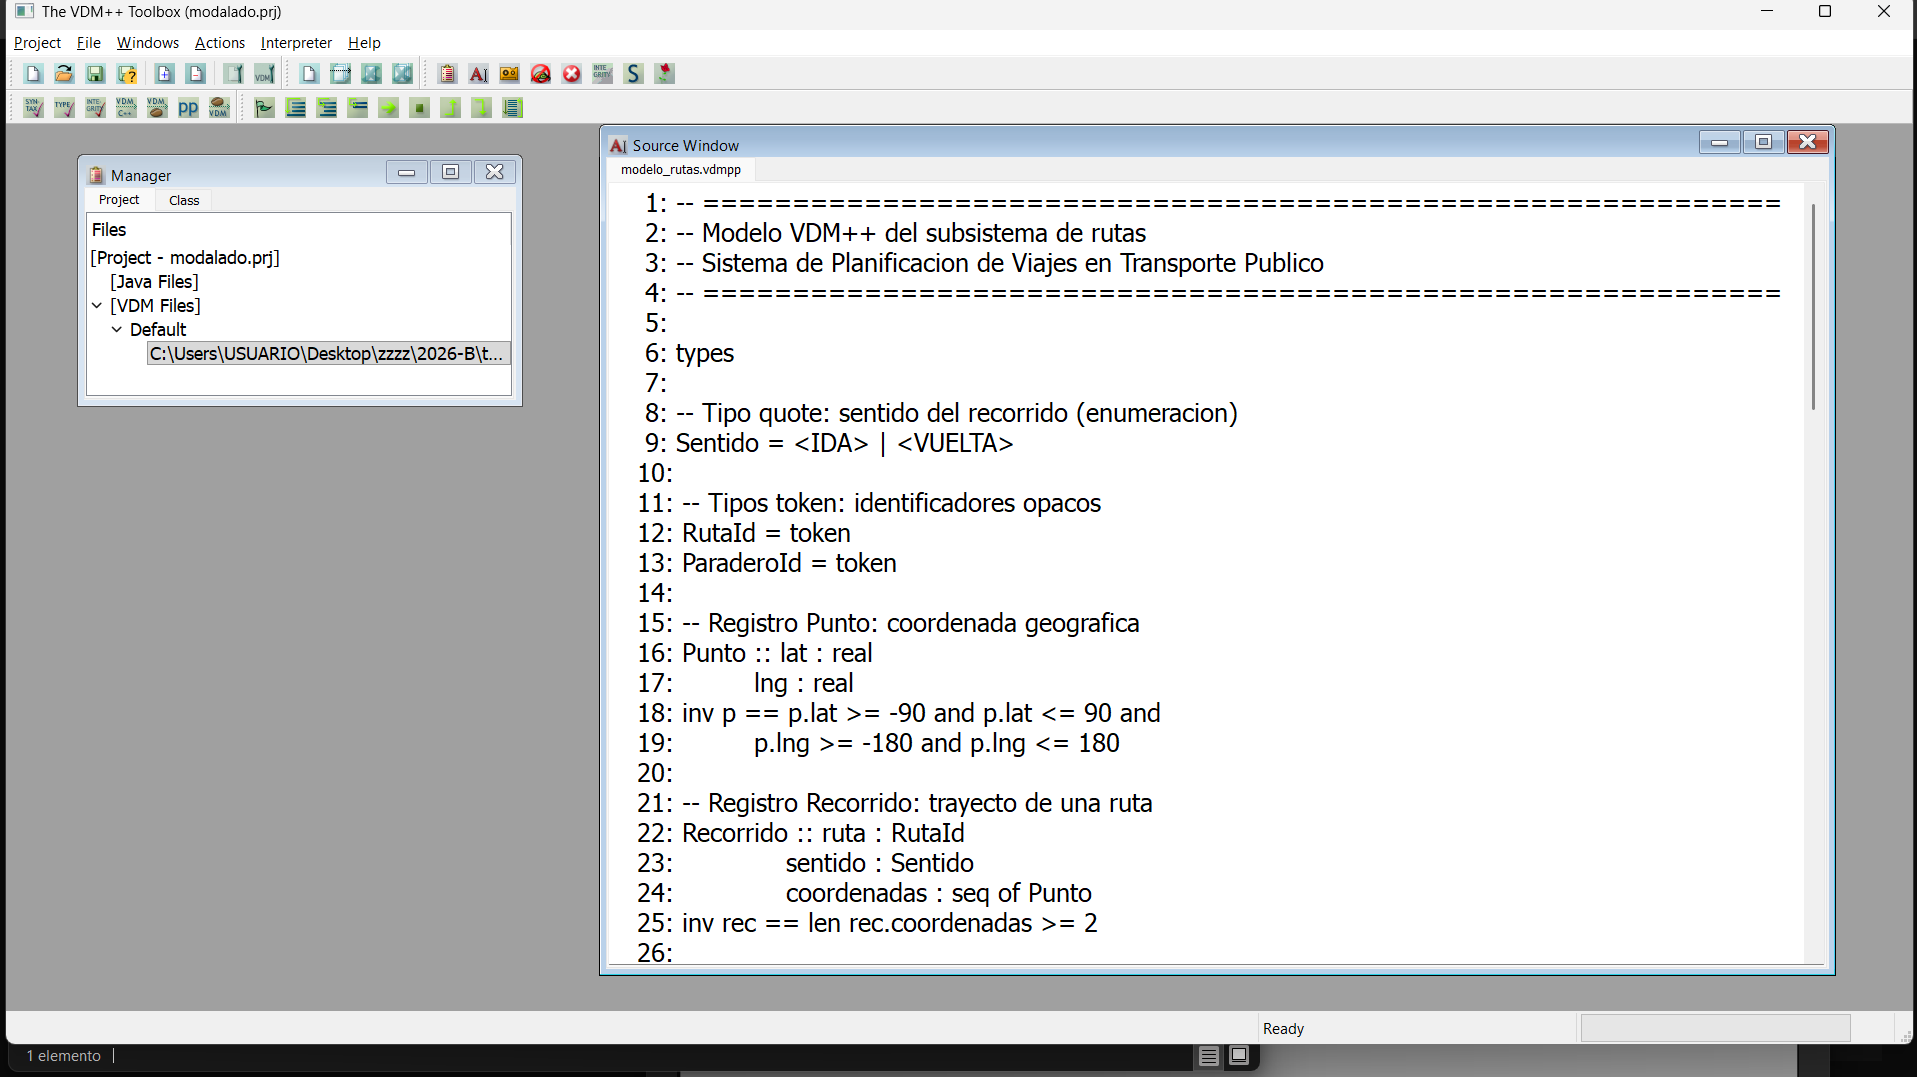
\includegraphics[width=0.82\textwidth]{images/Modelo_abierto_en_la_Toolbox.png}
\caption{Modelo VDM++ del subsistema de rutas cargado en la VDM++ Toolbox.}
\label{fig:modelo}
\end{figure*}

\subsection{Tipos e invariantes}
\label{sec:tipos}

El modelo define el tipo \emph{quote} \texttt{Sentido} (ida o vuelta), el
identificador de ruta \texttt{RutaId}, y los tipos compuestos
\texttt{Punto} (coordenada geográfica) y \texttt{Recorrido} (ruta, sentido
y secuencia de puntos):

\begin{lstlisting}
class Sistema
types
  public Sentido   = <IDA> | <VUELTA>;
  public RutaId    = nat;
  public Punto     = real * real;
  public Recorrido = RutaId * Sentido * seq of Punto;

instance variables
  recorridos : set of Recorrido := {};
\end{lstlisting}

El dominio impone dos invariantes: (i) todo punto debe tener coordenadas
dentro del rango geográfico válido ($-90^{\circ} \le lat \le 90^{\circ}$ y
$-180^{\circ} \le lng \le 180^{\circ}$); y (ii) todo recorrido debe tener
al menos dos puntos, pues un trayecto requiere origen y destino. Estas
propiedades se documentan en el modelo y se reflejan en las precondiciones
de las funciones auxiliares y en los datos de prueba.

\subsection{Operaciones y postcondiciones}
\label{sec:operaciones}

Sobre la variable de instancia \texttt{recorridos : set of Recorrido} se
definen las operaciones de búsqueda. \texttt{buscarRutasDirectas} (RF1)
devuelve los recorridos que pasan a una distancia menor o igual a
\texttt{radio} del origen \texttt{A} y del destino \texttt{B}:

\begin{lstlisting}
public buscarRutasDirectas : Punto * Punto * real ==> set of Recorrido
buscarRutasDirectas(A, B, radio) ==
  return { rec | rec in set recorridos &
       cercaniaPunto(A, rec.#3) <= radio and
       cercaniaPunto(B, rec.#3) <= radio }
pre A <> B
post forall rec in set RESULT &
       cercaniaPunto(A, rec.#3) <= radio and
       cercaniaPunto(B, rec.#3) <= radio;
\end{lstlisting}

La postcondición formaliza la propiedad central: toda ruta devuelta se
encuentra a una distancia menor o igual al radio respecto del origen y
del destino. La operación \texttt{buscarRutasCombinadas} (RF2) extiende
la búsqueda a pares de recorridos conectados por un transbordo; su
postcondición exige además que las rutas sean distintas y que exista un
punto de transbordo dentro de \texttt{radioTransbordo}.

\subsection{Diagrama de clases}
\label{sec:clases}

La Figura~\ref{fig:clases} presenta el diagrama de clases del dominio de
rutas. Una empresa posee varias rutas; cada ruta tiene uno o dos
recorridos (ida y vuelta); y cada recorrido se asocia con paraderos a
través de la clase \texttt{RecorridoParadero}, que registra el orden y la
distancia.

\begin{figure*}[!t]
\centering
\resizebox{0.95\textwidth}{!}{%
\begin{tikzpicture}[
  class/.style={draw, rectangle, rounded corners=2pt, align=left, inner sep=5pt, font=\small},
  assoc/.style={-{Stealth[length=2mm]}, thick}
]
\node[class] (empresa) at (0,4) {\begin{tabular}{l}\textbf{Empresa}\\\hline nombre\\descripcion\end{tabular}};
\node[class] (ruta) at (3.6,4) {\begin{tabular}{l}\textbf{Ruta}\\\hline nombre\\codigo\end{tabular}};
\node[class] (recorrido) at (8.2,4) {\begin{tabular}{l}\textbf{Recorrido}\\\hline sentido : Sentido\\coordenadas : seq of Punto\end{tabular}};
\node[class] (paradero) at (13.8,4) {\begin{tabular}{l}\textbf{Paradero}\\\hline nombre\\latitud\\longitud\end{tabular}};
\node[class] (rpar) at (11.0,0.3) {\begin{tabular}{l}\textbf{RecorridoParadero}\\\hline orden : nat\\distancia : real\end{tabular}};
\draw[assoc] (empresa) -- (ruta) node[pos=0.15,above]{1} node[pos=0.85,above]{*};
\draw[assoc] (ruta) -- (recorrido) node[pos=0.15,above]{1} node[pos=0.85,above]{1..2};
\draw[assoc] (recorrido) -- (rpar) node[pos=0.3,left]{1} node[pos=0.72,right]{*};
\draw[assoc] (paradero) -- (rpar) node[pos=0.3,right]{1} node[pos=0.72,left]{*};
\end{tikzpicture}}
\caption{Diagrama de clases del dominio de rutas.}
\label{fig:clases}
\end{figure*}

El diagrama también se documenta en formato PlantUML, lo que permite
regenerarlo o exportarlo a otros formatos:

\begin{lstlisting}
@startuml
class Empresa { nombre; descripcion }
class Ruta { nombre; codigo }
class Recorrido { sentido; coordenadas }
class Paradero { nombre; latitud; longitud }
class RecorridoParadero { orden; distancia }
Empresa "1" --> "*" Ruta
Ruta "1" --> "1..2" Recorrido
Recorrido "1" --> "*" RecorridoParadero
Paradero "1" --> "*" RecorridoParadero
@enduml
\end{lstlisting}

La Figura~\ref{fig:typecheck} muestra que el análisis de tipos del modelo
finaliza sin errores.

\begin{figure*}[!t]
\centering
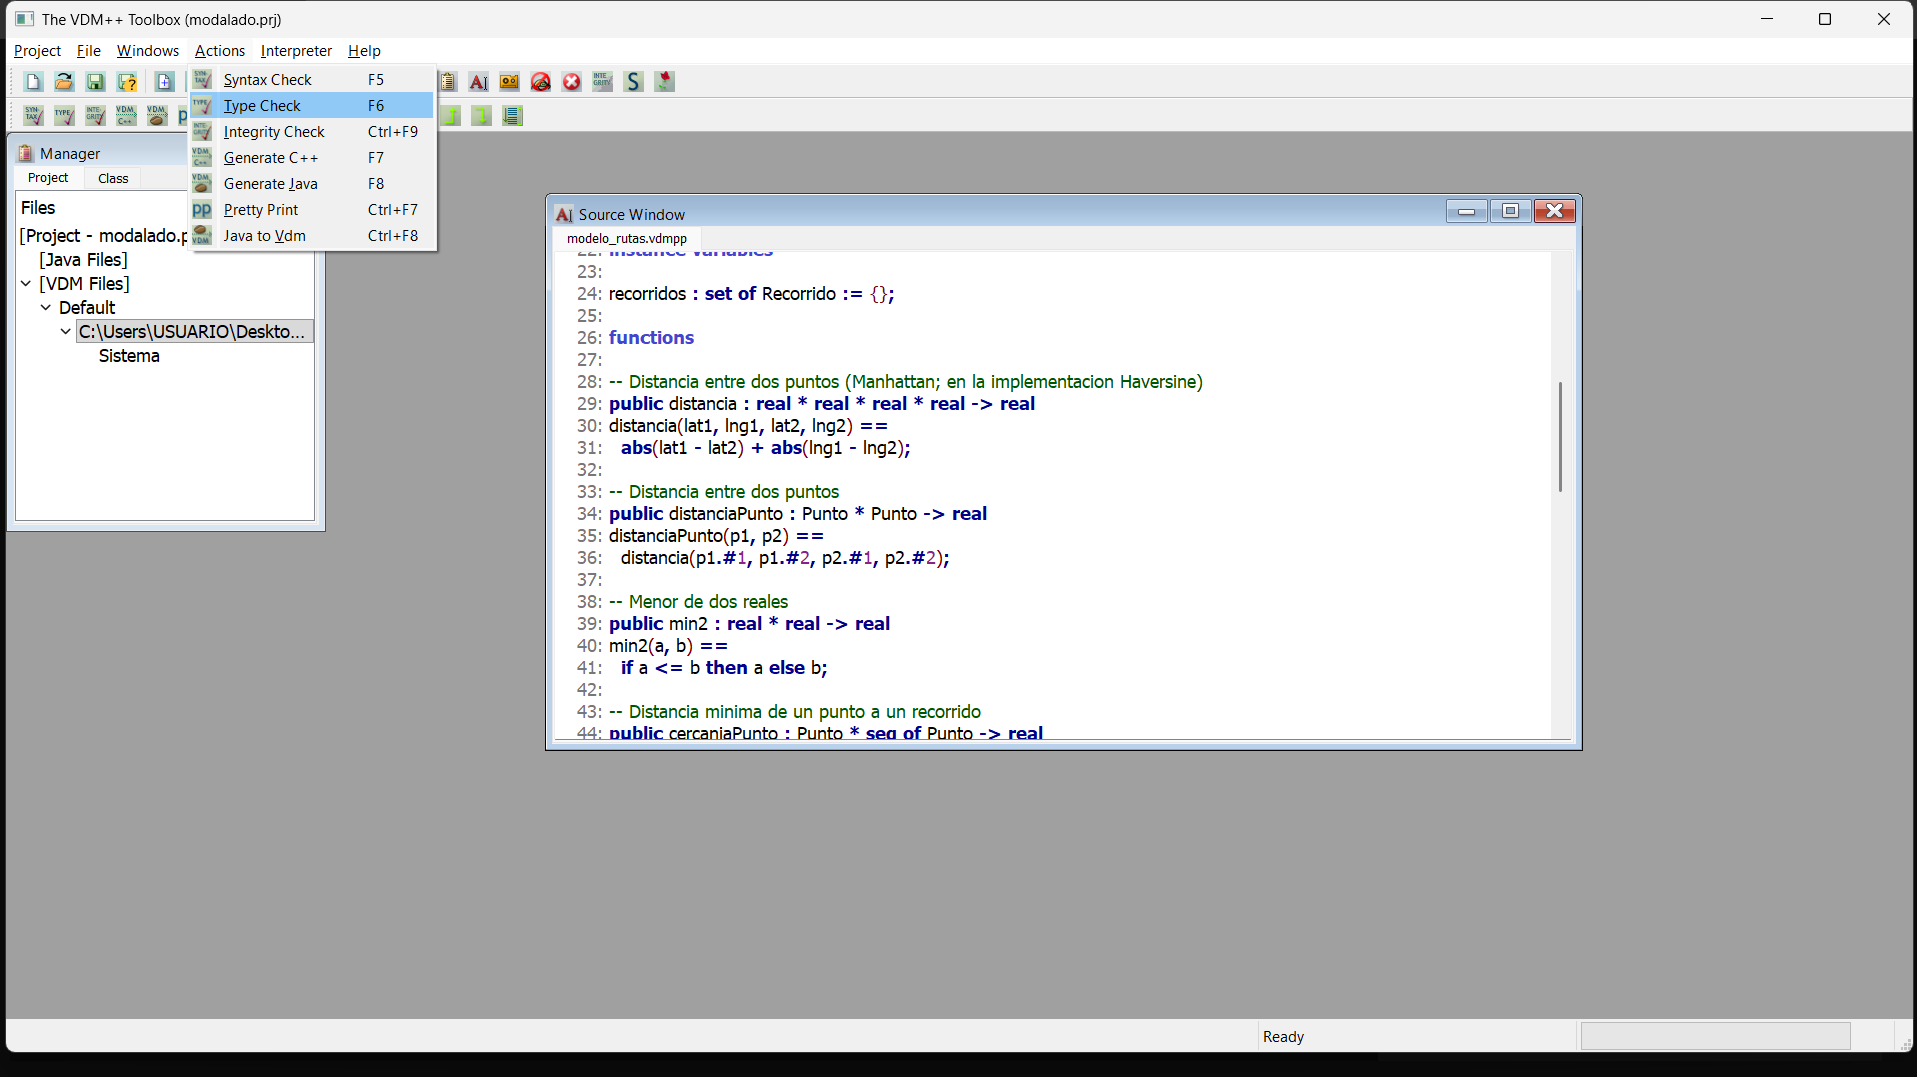
\includegraphics[width=0.82\textwidth]{images/Type_Check_sin_errores.png}
\caption{Análisis de tipos (\emph{type check}) del modelo sin errores.}
\label{fig:typecheck}
\end{figure*}
